%%%%(c)
%%%%(c)  This file is a portion of the source for the textbook
%%%%(c)
%%%%(c)    Abstract Algebra: Theory and Applications
%%%%(c)    Copyright 1997 by Thomas W. Judson
%%%%(c)
%%%%(c)  See the file COPYING.txt for copying conditions
%%%%(c)
%%%%(c)
\chap{Preliminaries}{sets}

%% TWJ, 2010/03/31
%% Chapters now begin with Chapter 1
 
\chapterletter{A}{ }certain amount of mathematical maturity is necessary to find and study applications of abstract algebra.  A basic knowledge of set theory, mathematical induction, equivalence relations, and matrices is a must.  Even more important is the ability to read and understand mathematical proofs.  In this chapter we will outline the background needed for a course in abstract algebra.
 

\section{A Short Note on Proofs}\label{sets_short_note}
 
Abstract mathematics is different from other sciences. In laboratory sciences such as chemistry and physics, scientists perform experiments to discover new principles and verify theories.  Although mathematics is often motivated by physical experimentation or by computer simulations, it is made rigorous through the use of logical arguments.  In studying abstract mathematics, we take what is called an  axiomatic approach; that is, we take a collection of objects $\mathcal S$ and assume some rules about their structure.  These rules are called {\bfi axioms}.  Using the axioms for $\mathcal S$, we wish to derive other information about $\mathcal S$ by using logical arguments.  We require that our axioms be consistent; that is, they should not contradict one another.  We also demand that there not be too many axioms.  If a system of axioms is too restrictive,  there will be few examples of the mathematical structure.  

A {\bfi statement\/} in logic or mathematics is an assertion that is either true or false.  Consider the following examples:
\begin{itemize}
 
\item
$3 + 56 - 13 + 8/2 $.
 
\item
All cats are black.
 
\item
$2 + 3 = 5$.
 
\item
$2x = 6$ exactly when $x = 4$.
 
\item
If $ax^2 + bx + c = 0$ and $a \neq 0$, then
\[
x = \frac{-b \pm \sqrt{b^2 - 4ac}}{2a}.
\]
 
\item
$x^3 - 4x^2 + 5 x - 6$.
 
\end{itemize}
All but the first  and last examples are statements, and must be either true or false.  
 
A {\bfi mathematical proof\/} is nothing more than a convincing argument about the accuracy  of a statement. Such an argument should contain enough detail to convince the audience; for instance, we can see that the statement ``$2x=6$ exactly when $x = 4$'' is false by evaluating $2 \cdot 4$ and noting that $6 \neq 8$, an argument that would satisfy anyone. Of course, audiences may vary widely: proofs can be addressed to another student, to a professor, or to the reader of a text.  If more detail than  needed is presented in the proof, then the  explanation will be either long-winded or poorly written.  If too much detail is omitted, then the proof may  not be convincing.  Again it is important to keep the audience in mind.  High school students require much more detail than do graduate students.  A good rule of thumb for an argument in an introductory abstract algebra course is that it should be written to convince one's peers, whether those peers be other students or other readers of the text. 

Let us examine different types of statements.  A statement could be as simple as ``$10/5 = 2$''; however, mathematicians are usually interested in more complex statements such as ``If $p$, then $q$,'' where $p$ and $q$ are both statements.  If certain statements are known or assumed to be true, we wish to know what we can say about other statements.  Here $p$ is called the {\bfi hypothesis\/} and $q$ is known as the {\bfi conclusion}.  Consider the following statement: If $ax^2 + bx + c = 0$ and $a \neq 0$, then  
\[
x = \frac{-b \pm \sqrt{b^2 - 4ac}}{2a}.
\]
The hypothesis is $ax^2 + bx + c = 0$ and $a \neq 0$; the conclusion is 
\[
x = \frac{-b \pm \sqrt{b^2 - 4ac}}{2a}.
\]
Notice that the  statement says nothing about whether or not the hypothesis is true. However, if this entire statement is true and we can show that $ax^2 + bx + c = 0$ with $a \neq 0$ is true, then the conclusion {\em must\/} be true.  A proof of this statement might simply be a series of equations: 
\begin{align*}
ax^2 + bx + c & =  0 \\
x^2 + \frac{b}{a}x & =  - \frac{c}{a} \\
x^2 + \frac{b}{a}x + \left( \frac{b}{2a} \right)^2 & =  \left( \frac{b}{2a} \right)^2 - \frac{c}{a} \\
\left(x + \frac{b}{2a} \right)^2 & =  \frac{b^2 - 4ac}{4a^2} \\
x + \frac{b}{2a}  & =  \frac{ \pm \sqrt{ b^2 -4ac}}{2a} \\
x & =  \frac{-b \pm \sqrt{b^2 - 4ac}}{2a}.
\end{align*}

If we can prove a statement true, then that statement is called a {\bfi proposition}.  A proposition of major importance is called a {\bfi theorem}.  Sometimes instead of proving a theorem or proposition all at once, we break the proof down into modules; that is, we prove several supporting propositions, which are called {\bfi lemmas}, and use the results of these propositions to prove the main result. If we can prove a proposition or a theorem, we will often, with very little effort, be able to derive other related propositions called {\bfi corollaries}. 
 
 
\subsection*{Some Cautions and Suggestions}
 
There are several different strategies for proving propositions.  In addition to using different methods of proof, students often make some common mistakes when they are first learning how to prove theorems. To aid students who are studying abstract mathematics for the first time, we list here some of the difficulties that they may encounter and some of the strategies of proof available to them. It is a good idea to keep referring back to this list as a reminder. (Other techniques of proof will become apparent throughout this chapter and the remainder of the text.) 
\begin{itemize}
 
\item
A theorem cannot be proved by example; however, the standard way to show that a statement is not a theorem is to provide a counterexample. 
 
\item
Quantifiers are important. Words and phrases such as {\em only}, {\em for all}, {\em for every}, and {\em for some\/} possess different meanings. 
 
\item
Never assume any hypothesis that is not explicitly stated in the theorem.  {\em You cannot take things for granted.} 
 
\item
Suppose you wish to show that an object {\em exists\/} and is {\em unique}.  First show that there actually is such an object.  To show that it is unique, assume that there are two such objects, say $r$ and $s$, and then show that $r = s$.
 
\item
Sometimes it is easier to prove the contrapositive of a statement.  Proving the statement ``If $p$, then $q$'' is exactly the same as proving the statement ``If not $q$, then not $p$.''
 
\item
Although it is usually better to find a direct proof of a theorem, this task  can sometimes be difficult. It may be easier to assume that the theorem that you are trying to prove is false, and to hope that in the course of your argument you are forced to make some statement that cannot possibly be true.
 
\end{itemize}

Remember that one of the main objectives of higher mathematics is proving theorems. Theorems are tools that make new and productive applications of mathematics possible.  We use examples to give insight  into existing theorems and to foster intuitions as to what new theorems might be true.  Applications, examples, and proofs are tightly interconnected---much more so than they may seem at first appearance.
 
 
\section{Sets and Equivalence Relations}\label{sets_equivalence}
 
 
\subsection*{Set Theory}
 
A {\bfi set\/} is a well-defined collection of objects; that is, it is defined in such a manner that we can determine for any given object $x$ whether or not $x$ belongs to the set.  The objects that belong to a set are called its {\bfi elements} or {\bfi members}. We will denote sets by capital letters, such as $A$ or $X$; if $a$ is an element of the set $A$, we write $a \in A$\label{sets_membership}.

A set is usually specified either by listing all of its elements inside a pair of braces or by stating the property that determines whether or not an object $x$ belongs to the set. We might write
\[
X = \{ x_1, x_2, \ldots, x_n \}
\]
for a set containing elements $x_1, x_2, \ldots, x_n$ or
\[
X = \{ x :x \mbox{ satisfies ${\mathcal P}$}\}
\]
if each $x$ in $X$ satisfies a certain property ${\mathcal P}$.  For example, if $E$ is the set of even positive integers, we can describe $E$ by writing either 
\[
E = \{2, 4, 6, \ldots \}
\quad \text{or} \quad
E = \{ x : x \mbox{ is an even integer and $x > 0$} \}.
\]
We write $2 \in E$ when we want to say that 2 is in the set $E$, and $-3 \notin E$ to say that $-3$ is not in the set $E$.

Some of the more important sets that we will consider are the following: 
\begin{gather*}
{\mathbb N}\label{sets_naturalnum}  = \{n: n \mbox{ is a natural number}\}  = \{1, 2, 3, \ldots \}; \\
{\mathbb Z}\label{sets_integers}  = \{n : n \mbox{ is an integer} \} = \{\ldots, -1, 0, 1,  2, \ldots \} ; \\
{\mathbb Q}\label{sets_rationals} = \{r : r \mbox{ is a rational number}\} = \{p/q : p, q \in {\mathbb Z} \mbox{ where $q \neq 0$}\}; \\
{\mathbb R}\label{sets_reals} = \{ x : x \mbox{ is a real number} \}; \\
{\mathbb C}\label{sets_complexnum} = \{z : z \mbox{ is a complex number}\}.
\end{gather*}

We find various relations between sets and can perform operations on sets.  A set $A$ is a {\bfi subset\/} of $B$, written $A \subset B$\label{sets_contain} or $B \supset A$, if every element of $A$ is also an element of $B$.  For example,  
\[
\{4,5,8\} \subset \{2, 3, 4, 5, 6, 7, 8, 9 \}
\]
and
\[
{\mathbb N} \subset {\mathbb Z} \subset {\mathbb Q} \subset {\mathbb R} \subset {\mathbb C}.
\]
Trivially, every set is a subset of itself.  A set $B$ is a {\bfi proper subset\/} of a set $A$ if $B \subset A$ but $B \neq A$. If $A$ is not a subset of $B$, we write $A \notsubset B$; for example, $\{4, 7, 9\} \notsubset \{2, 4, 5,  8, 9 \}$.  Two sets are {\bfi equal}, written $A = B$, if we can show that $A \subset B$ and $B \subset A$.  

It is convenient to have a set with no elements in it.  This set is called the {\bfi empty set\/} and is denoted by $\emptyset$\label{sets_emptyset}.  Note that the empty set is a subset of every set.  

To construct new sets out of old sets, we can perform certain operations: the {\bfi union\/} $A \cup B$ of two sets $A$ and $B$ is defined as  
\[
A \cup B\label{sets_union} = \{x : \mbox{ $x \in A$ or $x \in B$} \};
\]
the {\bfi intersection\/} of $A$ and $B$  is defined by
\[
A \cap B\label{sets_intersection} = \{x : \mbox{ $x \in A$ and $x \in B$} \}.
\]
If $A = \{1, 3, 5\}$ and $B = \{ 1, 2, 3, 9 \}$, then
\[
A \cup B = \{1, 2, 3, 5, 9 \}
\quad \text{and} \quad
A \cap B = \{ 1, 3 \}.
\]
We can consider the union and the intersection of more than two sets.  In this case we write 
\[
\bigcup_{i = 1}^{n} A_{i} = A_{1} \cup \ldots \cup A_n
\]
and
\[
\bigcap_{i = 1}^{n} A_{i} = A_{1} \cap \ldots \cap A_n
\]
for the union and intersection, respectively, of the collection of sets $A_1, \ldots A_n$.

When two sets have no elements in common, they are said to be {\bfi disjoint}; for example, if $E$ is the set of even integers and $O$ is the set of odd integers, then $E$ and $O$ are disjoint.  Two sets $A$ and $B$ are disjoint exactly when $A \cap B = \emptyset$. 

Sometimes we will work within one fixed set $U$, called the {\bfi universal set}.  For any set $A \subset U$, we define the {\bfi complement\/} of $A$, denoted by $A'$\label{sets_complement}, to be the set 
\[
A' = \{ x : \mbox{ $x \in U$ and $x \notin A$} \}.
\]

We define the {\bfi difference\/} of two sets $A$ and $B$ to be
\[
A \setminus B\label{sets_difference} = A \cap B'  = \{ x : \mbox{ $x \in A$ and $x \notin B$} \}.
\]

\begin{example}{operations}
Let ${\mathbb R}$ be the universal set and suppose that
\[
A = \{ x \in {\mathbb R} : 0 < x \leq 3 \}
\quad \text{and} \quad
B = \{ x \in {\mathbb R} : 2 \leq x < 4 \}.
\]
Then
\begin{align*}
A \cap B & =  \{ x \in {\mathbb R} : 2 \leq x \leq 3 \} \\
A \cup B & =  \{ x \in {\mathbb R} : 0 < x < 4 \} \\
A \setminus B & =  \{ x \in {\mathbb R} : 0 < x < 2  \} \\
A' & =  \{ x \in {\mathbb R} : \mbox{ $x \leq 0$ or $x > 3$
} \}.
\end{align*}
\end{example}
 
\begin{proposition}\label{sets_theorem_set_ops}
Let $A$, $B$, and $C$ be sets. Then
\begin{enumerate}
 
\rm\item\it
$A \cup A = A$, $A \cap A = A$, and $A \setminus A = \emptyset$;
 
\rm\item\it
$A \cup \emptyset = A$ and $A \cap \emptyset = \emptyset$;
 
\rm\item\it
$A \cup (B \cup C) = (A \cup B) \cup C$ and  $A \cap (B \cap C) = (A \cap B) \cap C$;
 
\rm\item\it
$A \cup B = B \cup A$ and $A \cap B = B \cap A$;
 
\rm\item\it
$A \cup (B \cap C) = (A \cup B) \cap (A \cup C)$;
 
\rm\item\it
$A \cap (B \cup C) = (A \cap B) \cup (A \cap C)$.
 
\end{enumerate}
\end{proposition}

\begin{proof}
We will prove (1) and (3) and leave the remaining results to be proven in the exercises. 

(1)
Observe that
\begin{align*}
A \cup A & =  \{ x : \mbox{ $x \in A$ or $x \in A$} \} \\
& =  \{ x : \mbox{ $x \in A$} \} \\
& =  A
\end{align*}
and
\begin{align*}
A \cap A & =  \{ x : \mbox{ $x \in A$ and $x \in A$} \} \\
& =  \{ x : \mbox{ $x \in A$}  \} \\
& =  A.
\end{align*}
Also, $A \setminus A = A \cap A' = \emptyset$.
 
(3)
For sets $A$, $B$, and $C$,
\begin{align*}
A \cup (B \cup C)
& =
A \cup \{ x : \mbox{ $x \in B$ or $x \in C$} \} \\
& =
\{ x : \mbox{ $x \in A$ or $x \in B$, or $x \in C$} \} \\
& =
\{ x : \mbox{ $x \in A$ or $x \in B$} \} \cup C \\
& =
(A \cup B) \cup C.
\end{align*}
A  similar argument proves that  $A \cap (B \cap C) = (A \cap B) \cap
C$. 
\end{proof}

\begin{theorem}[De Morgan's Laws]\index{De Morgan's laws!for sets}\label{sets_de_morgan}
Let $A$ and $B$ be sets. Then 
\begin{enumerate}
 
\rm\item\it
$(A \cup B)' = A' \cap B'$; 
 
\rm\item\it
$(A \cap B)' = A' \cup B'$.
 
\end{enumerate}
\end{theorem}
 
\begin{proof}
(1) 
We must show that $(A \cup B)' \subset A' \cap B'$ and $(A \cup B)' \supset A' \cap B'$. Let $x \in (A \cup B)'$.  Then $x \notin A \cup B$. So $x$ is neither in $A$ nor in $B$, by the definition of the union of sets.  By the definition of the complement, $x \in A'$ and $x \in B'$.  Therefore, $x \in A' \cap B'$ and we have $(A \cup B)' \subset A' \cap B'$.
 
To show the reverse inclusion, suppose that $x \in A' \cap B'$.  Then $x \in A'$ and $x \in B'$, and so $x \notin A$ and $x \notin B$.  Thus $x \notin A \cup B$ and so $x \in (A \cup B)'$.  Hence, $(A \cup B)' \supset A' \cap B'$ and so $(A \cup B)' = A' \cap B'$. 

The proof of (2) is left as an exercise.
\end{proof}
 
\begin{example}{other_relations}
Other relations between sets often hold true.  For example,
\[
( A \setminus B) \cap (B \setminus A) = \emptyset.
\]
To see that this is true, observe that
\begin{align*}
( A \setminus B) \cap (B \setminus A)
& =
( A \cap B') \cap (B \cap A') \\
& =
A \cap A' \cap B \cap B' \\
& = \emptyset.
\end{align*}
\end{example}
 
 
\subsection*{Cartesian Products and Mappings}

Given sets $A$ and $B$, we can define a new set $A \times\label{sets_cartesian} B$, called the {\bfi Cartesian product\/}  of $A$ and $B$, as a set of ordered pairs.  That is, 
\[
A \times B = \{ (a,b) : \mbox{ $a \in A$ and $b \in B$} \}.
\]

 
\begin{example}{cartesian_products}
If $A = \{ x, y \}$, $B = \{ 1, 2, 3 \}$, and $C = \emptyset$, then $A \times B$ is the set 
\[
\{ (x, 1), (x, 2), (x, 3), (y, 1), (y, 2), (y, 3) \}
\]
and
\[
A \times C = \emptyset.
\]
\end{example}

We define the {\bfi Cartesian product of $n$ sets\/} to be
\[
A_1 \times \cdots \times A_n = \{ (a_1, \ldots, a_n): a_i \in A_i {\rm\; for\;} i = 1, \ldots, n \}.
\]
If $A = A_1 = A_2 = \cdots = A_n$, we often write $A^n$ for $A \times \cdots \times A$ (where $A$ would be written $n$ times)\label{sets_ncartesian}.   For example, the set ${\mathbb R}^3$ consists of all of 3-tuples of real numbers.
 
Subsets of $A \times B$ are called {\bfi relations}.  We will define a  {\bfi mapping\/}\index{Mapping|see{Function}} or {\bfi function}\index{Function!definition of} $f \subset A \times B$ from a set $A$ to a set $B$ to be the special type of  relation in which for each element $a \in A$ there is a unique element $b \in B$ such that $(a, b) \in f$; another way of saying this is that for every element in $A$, $f$ assigns a unique element in $B$.  We usually write $f:A \rightarrow B$ or $A \stackrel{f}{\rightarrow} B$.  Instead of writing down ordered pairs  $(a,b) \in A \times B$, we write $f(a) = b$ or $f : a \mapsto b$.  The set  $A$ is called the {\bfi domain\/}\index{Function!domain of} of $f$ and   
\[
f(A) = \{ f(a) : a \in A \} \subset B
\]
is called the {\bfi range\/}\index{Function!range of} or {\bfi image\/} of $f$.  We can think of the elements in the function's domain as input values and the elements in the function's range as output values.  
 
\begin{figure}[htb] %Changed the figure to a tikz diagram - TWJ 5/4/2010

\begin{center}
%\includegraphics[width=2.5in]{sets_figure_mappings} \\
\tikzpreface{sets_mappings}
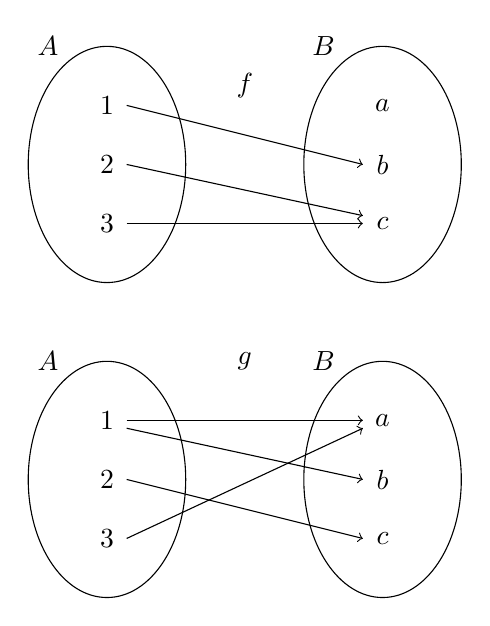
\begin{tikzpicture}[scale=0.5]
\draw (0,0) ellipse (2 and 3);
\draw (7,0) ellipse (2 and 3);
\draw (0,8) ellipse (2 and 3);
\draw (7,8) ellipse (2 and 3);
\draw [->] (0.5,9.5) -- (6.5,8);
\draw [->] (0.5,8) -- (6.5,6.7);
\draw [->] (0.5,6.5) -- (6.5,6.5);
\draw [->] (0.5,1.5) -- (6.5,1.5);
\draw [->] (0.5,1.3) -- (6.5,0);
\draw [->] (0.5,0) -- (6.5,-1.5);
\draw [->] (0.5,-1.5) -- (6.5,1.3);
\node at (0, 1.5) {1};
\node at (0, 0) {2};
\node at (0, -1.5) {3};
\node at (7, 1.5) {$a$};
\node at (7, 0) {$b$};
\node at (7, -1.5) {$c$};
\node at (0, 9.5) {1};
\node at (0, 8) {2};
\node at (0, 6.5) {3};
\node at (7, 9.5) {$a$};
\node at (7, 8) {$b$};
\node at (7, 6.5) {$c$};
\node at (-1.5,11) {$A$};
\node at (5.5,11) {$B$};
\node at (-1.5,3) {$A$};
\node at (5.5,3) {$B$};
\node at (3.5,3) {$g$};
\node at (3.5,10) {$f$};
\end{tikzpicture}

\caption{Mappings} \label{sets_figure_mappings} 

\end{center}
\end{figure}

\begin{example}{mappings}
Suppose $A = \{1, 2, 3 \}$ and $B = \{a, b, c \}$.  In Figure~\ref{sets_figure_mappings} we define relations $f$ and  $g$ from $A$ to $B$.  The relation $f$ is a mapping, but $g$ is not because $1 \in A$ is not assigned to a unique element in $B$; that is, $g(1) = a$ and $g(1) = b$.  
\end{example}

Given a function $f : A \rightarrow B$, it is often possible to write a list describing what the function does to each specific element in the domain.  However, not all functions can be described in this manner.  For example, the function $f: {\mathbb R} \rightarrow {\mathbb R}$ that sends each real number to its cube is a mapping that must be described by writing $f(x) = x^3$ or $f:x \mapsto x^3$. 
 
Consider the relation $f : {\mathbb Q} \rightarrow {\mathbb Z}$ given by $f(p/q) = p$.  We know that $1/2 = 2/4$, but is $f(1/2) = 1$ or 2?  This relation cannot be a mapping because it is not well-defined.  A relation is {\bfi well-defined\/}\index{Well-defined map} if each element in the domain is assigned to a {\em unique\/} element in the range. 

If $f:A \rightarrow B$ is a map and the image of $f$ is $B$, i.e., $f(A) = B$, then $f$ is said to be {\bfi onto\/}\index{Function!onto} or {\bfi surjective}\index{Function!surjective}.  A map is {\bfi one-to-one\/}\index{Function!one-to-one} or {\bfi injective\/}\index{Function!injective} if $a_1 \neq a_2$ implies $f(a_1) \neq f(a_2)$.  Equivalently, a function is one-to-one if $f(a_1) = f(a_2)$ implies $a_1 = a_2$.  A map that is both one-to-one and onto is called {\bfi bijective}\index{Function!bijective}.

\begin{example}{one_to_one_onto}
Let $f:{\mathbb Z} \rightarrow {\mathbb Q}$ be defined by $f(n) = n/1$.  Then $f$ is one-to-one but not onto.  Define $g : {\mathbb Q} \rightarrow {\mathbb Z}$ by $g(p/q) = p$ where $p/q$ is a rational number expressed in its lowest terms with a positive denominator.  The function $g$ is onto but not one-to-one. 
\end{example}

Given two functions, we can construct a new function by using the range of the first function as the domain of the second function.  Let $f : A \rightarrow B$ and $g : B \rightarrow C$ be mappings.  Define a new map, the {\bfi composition\/}\index{Function!composition of} of $f$ and $g$ from $A$ to $C$, by $(g \circ f)(x) = g(f(x))$.

\begin{figure}[htb]\label{sets_figure_composition} %Changed the figure to a tikz diagram - TWJ 5/4/2010
\begin{center}
\caption{Composition of maps}
\bigskip
%\includegraphics[width=3.5in]{sets_figure_composition}
\tikzpreface{sets_composition}
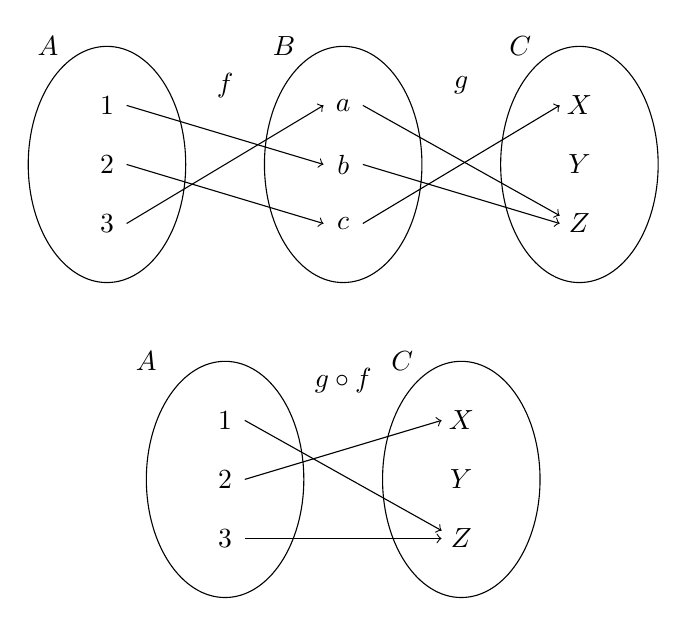
\begin{tikzpicture}[scale=0.5]
\draw (-6,8) ellipse (2 and 3);
\draw (0,8) ellipse (2 and 3);
\draw (6,8) ellipse (2 and 3);

\node at (-7.5,11) {$A$};
\node at (-1.5,11) {$B$};
\node at (4.5,11) {$C$};
\node at (-6, 9.5) {1};
\node at (-6, 8) {2};
\node at (-6, 6.5) {3};
\node at (0, 9.5) {$a$};
\node at (0, 8) {$b$};
\node at (0, 6.5) {$c$};
\node at (6, 9.5) {$X$};
\node at (6, 8) {$Y$};
\node at (6, 6.5) {$Z$};
\node at (-3,10) {$f$};
\node at (3,10) {$g$};

\draw [->] (0.5,9.5) -- (5.5,6.7);
\draw [->] (0.5,8) -- (5.5,6.5);
\draw [->] (0.5,6.5) -- (5.5,9.5);

\draw [->] (-5.5,9.5) -- (-0.5,8);
\draw [->] (-5.5,8) -- (-0.5,6.5);
\draw [->] (-5.5,6.5) -- (-0.5,9.5);


\draw (-3,0) ellipse (2 and 3);
\draw (3,0) ellipse (2 and 3);

\node at (-5,3) {$A$};
\node at (1.5,3) {$C$};
\node at (-3, 1.5) {1};
\node at (-3, 0) {2};
\node at (-3, -1.5) {3};
\node at (3, 1.5) {$X$};
\node at (3, 0) {$Y$};
\node at (3, -1.5) {$Z$};
\node at (0,2.5) {$g \circ f$};

\draw [->] (-2.5,1.5) -- (2.5,-1.3);
\draw [->] (-2.5,0) -- (2.5,1.5);
\draw [->] (-2.5,-1.5) -- (2.5,-1.5);

\end{tikzpicture}
\end{center}
\end{figure}

\begin{example}{composition}
Consider the functions $f: A \rightarrow B$ and $g: B \rightarrow C$ that are defined in Figure~\ref{sets_figure_composition}(a).  The composition of these functions, $g \circ f: A \rightarrow C$, is defined in
Figure~\ref{sets_figure_composition}(b). 
\end{example}

\begin{example}{composition_noncommute}
Let $f(x) = x^2$ and $g(x) = 2x + 5$. Then
\[
(f \circ g)(x) = f(g(x)) = (2x + 5)^2 = 4x^2 + 20x + 25 
\]
and
\[
(g \circ f)(x) = g(f(x)) = 2x^2 + 5.
\]
In general, order makes a difference; that is, in most cases $f \circ g \neq g \circ f$. 
\end{example}
 
\begin{example}{composition_commute}
Sometimes it is the case that $f \circ g= g \circ f$.  Let $f(x) = x^3$ and $g(x) = \sqrt[3]{x}$. Then 
\[
(f \circ g )(x) = f(g(x)) = f( \sqrt[3]{x}\, ) = (\sqrt[3]{x}\, )^3 = x
\]
and
\[
(g \circ f )(x) = g(f(x)) = g( x^3) = \sqrt[3]{ x^3} = x.
\]
\end{example}
 
\begin{example}{linear_map}
Given a $2 \times 2$ matrix
\[
A =
\begin{pmatrix}
a & b \\
c & d
\end{pmatrix},
\]
we can define a map $T_A : {\mathbb R}^2 \rightarrow {\mathbb R}^2$ by 
\[
T_A (x,y) = (ax + by, cx +dy)
\]
for $(x,y)$ in ${\mathbb R}^2$.  This is actually matrix multiplication; that is,
\[
\begin{pmatrix}
a & b \\
c & d
\end{pmatrix}
\begin{pmatrix}
x \\ y
\end{pmatrix}
=
\begin{pmatrix}
ax + by \\
cx +dy
\end{pmatrix}.
\]
Maps from ${\mathbb R}^n$ to ${\mathbb R}^m$ given by matrices are called {\bfi linear maps\/} or {\bfi linear transformations}\index{Linear transformation!definition of}.
\end{example}

\begin{example}{permutation}
Suppose that $S = \{ 1,2,3  \}$. Define a map $\pi :S\rightarrow S$ by 
\[
\pi( 1 )  = 2, \qquad
\pi( 2 )  = 1, \qquad
\pi( 3 )  = 3.
\]
This is a bijective map.  An alternative way to  write $\pi$ is
\[
\begin{pmatrix}
1 & 2 & 3 \\
\pi(1) & \pi(2) & \pi(3)
\end{pmatrix}
=
\begin{pmatrix}
1 & 2 & 3 \\
2 & 1 & 3
\end{pmatrix}.
\]
For any set $S$, a one-to-one and onto mapping $\pi : S \rightarrow S$ is called a {\bfi permutation\/}\index{Permutation!definition of} of $S$. 
\end{example}

\begin{theorem}\label{sets_theorem_mapping_properties}
Let $f : A \rightarrow B$, $g : B \rightarrow C$, and $h : C \rightarrow D$. Then  
\begin{enumerate}
 
\rm\item\it
The composition of mappings is associative; that is, $(h \circ g) \circ f = h \circ (g \circ f)$;  
 
\rm\item\it
If $f$ and $g$ are both one-to-one, then the mapping $g \circ f$ is one-to-one; 
 
\rm\item\it
If $f$ and $g$ are both onto, then the mapping $g \circ f$ is onto;  
 
\rm\item\it
If $f$ and $g$ are bijective, then so is $g \circ f$.
 
\end{enumerate}
\end{theorem}
 
\begin{proof}
We will prove (1) and (3). Part (2) is left as an exercise.  Part (4) follows directly from (2) and (3). 
 
(1) 
We must show that
\[
h \circ (g \circ f) = (h \circ g) \circ f.
\]
For $a \in A$ we have
\begin{align*}
(h \circ (g \circ f))(a) & = h((g \circ f)(a)) \\
& = h(g(f(a)))  \\
& = (h \circ g)(f(a)) \\
& = ((h \circ g) \circ f)(a).
\end{align*}
 
(3) 
Assume that $f$ and $g$ are both onto functions.  Given $c \in C$, we must show that there exists an $a \in A$ such that $(g \circ f)(a) = g(f(a)) = c$.  However, since $g$ is onto, there is a $b \in B$ such that $g(b) = c$.  Similarly, there is an $a \in A$ such that $f(a) = b$.  Accordingly, 
\[
(g \circ f)(a) = g(f(a)) = g(b) = c.
\]
\end{proof}
 
\medskip
 
If $S$ is any set, we will use $id_S$ or $id$\label{sets_identity} to denote the {\bfi identity mapping\/}\index{Function!identity} from $S$ to itself.  Define this map by $id(s) = s$ for all $s \in S$.  A map $g: B \rightarrow A$ is an {\bfi inverse mapping\/} of $f: A \rightarrow B$ if $g \circ f = id_A$ and $f \circ g = id_B$; in other words, the inverse function of a function simply ``undoes'' the function.   A map is said to be {\bfi invertible\/}\index{Function!invertible} if it has an inverse.  We usually write $f^{-1}$ for the inverse of $f$.  

\begin{example}{inverse_function}
The function $f(x) = x^3$ has inverse $f^{-1}(x) = \sqrt[3]{x}$ by Example~\ref{example:sets:composition_commute}. 
\hspace*{1in}
\end{example}

\begin{example}{exponential}
The natural logarithm and the exponential functions, $f(x) = \ln x$ and $f^{-1}(x) = e^x$, are inverses of each other provided that we are careful about choosing domains.  Observe that  
\[
f(f^{-1}(x)) = f(e^x) = \ln e^x = x
\]
and
\[
f^{-1}(f(x)) = f^{-1}(\ln x) = e^{\ln x} = x
\]
whenever composition makes sense.
\end{example}

\begin{example}{inverse_matrix}
Suppose that
\[
A =
\begin{pmatrix}
3 & 1 \\
5 & 2
\end{pmatrix}.
\]
Then $A$ defines a map from ${\mathbb R}^2$ to ${\mathbb R}^2$ by
\[
T_A (x,y) = (3x +  y, 5x +2y).
\]
We can find an inverse map of $T_A$ by simply inverting the matrix $A$; that is, $T_A^{-1} = T_{A^{-1}}$. In this example,
\[
A^{-1} =
\begin{pmatrix}
2  & -1 \\
-5 &  3
\end{pmatrix};
\]
hence, the inverse map is given by
\[
T_A^{-1} (x,y) = (2x -  y, -5x + 3y).
\]
It is easy to check that
\[
T^{-1}_A \circ T_A (x,y) = T_A \circ T_A^{-1} (x,y) = (x,y).
\]
Not every map has an inverse.  If we consider the map
\[
T_B (x,y) = (3x , 0 )
\]
given by the matrix
\[
B =
\begin{pmatrix}
3 & 0 \\
0 & 0
\end{pmatrix},
\]
then an inverse map would have to be of the form
\[
T_B^{-1} (x,y) = (ax + by, cx +dy)
\]
and
\[
(x,y) = T \circ T_B^{-1} (x,y) = (3ax + 3by, 0)
\]
for all $x$ and $y$.  Clearly this is  impossible because $y$ might not be 0. 
\end{example}

\begin{example}{inverse_permutation}
Given the permutation
\[
\pi =
\begin{pmatrix}
1 & 2 & 3 \\
2 & 3 & 1
\end{pmatrix}
\]
on $S = \{ 1,2,3 \}$, it is easy to see that the permutation defined by
\[
\pi^{-1} =
\begin{pmatrix}
1 & 2 & 3 \\
3 & 1 & 2
\end{pmatrix}
\]
is the inverse of $\pi$.  In fact, any bijective mapping possesses an inverse, as we will see in the next theorem.
\end{example}
 
\begin{theorem}\label{sets_theorem_invertible_maps}
A mapping is invertible if and only if it is both one-to-one and onto. 
\end{theorem}

\begin{proof}
Suppose first that $f:A \rightarrow B$ is invertible with inverse $g: B \rightarrow A$. Then $g \circ f = id_A$ is the identity map; that is, $g(f(a)) = a$. If $a_1, a_2 \in A$ with $f(a_1) = f(a_2)$, then $a_1 = g(f(a_1)) = g(f(a_2)) = a_2$.  Consequently, $f$ is one-to-one.  Now suppose that $b \in B$. To show that $f$ is onto, it is necessary to find an $a \in A$ such that $f(a) = b$, but $f(g(b)) = b$ with $g(b) \in A$. Let $a = g(b)$. 

Now assume the converse; that is, let $f$ be bijective.  Let $b \in B$.  Since $f$ is onto, there exists an $a \in A$ such that $f(a) = b$.  Because $f$ is one-to-one, $a$ must be unique. Define $g$ by letting $g(b) = a$.  We have now constructed the inverse of $f$.
\end{proof}
 

\subsection*{Equivalence Relations and Partitions}

A fundamental notion in mathematics is that of equality.  We can generalize equality with the introduction of equivalence relations and equivalence classes.  An {\bfi equivalence relation\/}\index{Equivalence relation} on a set $X$ is a relation $R \subset X \times X$ such that  
\begin{itemize}
 
\item
$(x, x) \in R$ for all $x \in X$ ({\bfi reflexive property});
  
\item
$(x, y) \in R$ implies $(y, x) \in R$ ({\bfi symmetric property});
 
\item
$(x, y)$ and $(y, z) \in R$ imply $(x, z) \in R$ ({\bfi transitive property}).
 
\end{itemize}
Given an equivalence relation $R$  on a set $X$, we usually write  $x \sim y$ instead of $(x, y) \in R$.  If the equivalence relation already has an associated notation such as $=$, $\equiv$, or $\cong$, we will
use that notation. 

\begin{example}{equivalent_fractions}
Let $p$, $q$, $r$, and $s$ be integers, where $q$ and $s$ are nonzero.  Define $p/q \sim r/s$ if $ps = qr$.  Clearly $\sim$ is reflexive and symmetric.  To show that it is also transitive, suppose that $p/q \sim r/s$ and $r/s \sim t/u$, with $q$, $s$, and $u$ all nonzero.  Then $ps = qr$ and $ru = st$. Therefore, 
\[
psu = qru = qst.
\]
Since $s \neq 0$, $pu = qt$. Consequently, $p/q \sim t/u$.
\end{example}

\begin{example}{equivalent_derivative}
Suppose that $f$ and $g$ are differentiable functions on ${\mathbb R}$.  We can define an equivalence relation on such functions by letting $f(x) \sim g(x)$ if $f'(x) = g'(x)$. It is clear that $\sim$ is both reflexive and symmetric.  To demonstrate transitivity, suppose that $f(x) \sim g(x)$ and  $g(x) \sim h(x)$.  From calculus we know that $f(x) - g(x) = c_1$ and $g(x)- h(x) = c_2$, where $c_1$ and $c_2$ are both constants. Hence, 
\[
f(x) - h(x) = ( f(x) - g(x)) + ( g(x)- h(x))  = c_1 - c_2
\]
and $f'(x) - h'(x) =0$. Therefore, $f(x) \sim h(x)$.
\end{example}

\begin{example}{equivalent_circles}
For $(x_1, y_1 )$ and $(x_2, y_2)$ in ${\mathbb R}^2$, define $(x_1, y_1 ) \sim (x_2, y_2)$ if $x_1^2 + y_1^2 = x_2^2 + y_2^2$.  Then $\sim$ is an equivalence relation on ${\mathbb R}^2$.
\end{example}

\begin{example}{equivalent_matrices}
Let $A$ and $B$ be \mbox{$2 \times 2$} matrices with entries in the real numbers. We can define an equivalence relation on the set of $2 \times 2$ matrices, by saying $A \sim B$ if there exists an invertible matrix $P$ such that $PAP^{-1} = B$.  For example, if 
\[
A =
\begin{pmatrix}
1 & 2 \\
-1 & 1
\end{pmatrix}
\quad \text{and} \quad
B =
\begin{pmatrix}
-18 & 33 \\
-11 & 20
\end{pmatrix},
\]
then $A \sim B$ since $PAP^{-1} = B$ for
\[
P =
\begin{pmatrix}
2 & 5 \\
1 & 3
\end{pmatrix}.
\]
Let $I$ be the $2 \times 2$ identity matrix; that is,
\[
I =
\begin{pmatrix}
1 & 0 \\
0 & 1
\end{pmatrix}.
\]
Then $IAI^{-1} = IAI = A$; therefore, the relation is reflexive.  To show symmetry, suppose that $A \sim B$.  Then there exists an invertible matrix $P$ such that $PAP^{-1} = B$.  So 
\[
A = P^{-1} B P = P^{-1} B (P^{-1})^{-1}.
\]
Finally, suppose that $A \sim B$ and $B \sim C$.  Then there exist invertible matrices $P$ and $Q$ such that $PAP^{-1} = B$ and  $QBQ^{-1} = C$.  Since 
\[
C = QBQ^{-1} = QPAP^{-1} Q^{-1} = (QP)A(QP)^{-1},
\]
the relation is transitive.  Two matrices that are equivalent in this manner are said to be {\bfi similar}\index{Matrix!similar}. 
\end{example}

A {\bfi partition}\index{Partitions} ${\mathcal P}$ of a set $X$ is a collection of nonempty sets $X_1, X_2, \ldots$ such that $X_i \cap X_j = \emptyset$ for $i  \neq j$ and $\bigcup_k X_k = X$. Let $\sim$ be an equivalence relation on a set $X$ and let $x \in X$.  Then $[x] = \{ y \in X : y \sim x \}$ is called the {\bfi equivalence class\/}\index{Equivalence class} of $x$.  We will see that an equivalence relation gives rise to a partition via equivalence classes.  Also, whenever a partition of a set exists, there is some natural  underlying equivalence relation, as the following theorem demonstrates.  
 
\begin{theorem}\label{sets_theorem_partitions}
Given an equivalence relation $\sim$ on a set $X$, the equivalence classes of $X$ form a partition of $X$.  Conversely, if ${\mathcal P} = \{ X_i\}$ is a partition of a set $X$, then there is an equivalence relation on $X$ with equivalence classes $X_i$. 
\end{theorem}

\begin{proof}
Suppose there exists an equivalence relation $\sim$ on the set $X$.  For any $x \in X$, the reflexive property shows that $x \in [x]$ and so $[x]$ is nonempty.  Clearly $X = \bigcup_{x \in X} [x]$.  Now let $x, y \in X$. We need to show that either $[x] = [y]$ or $[x] \cap [y] = \emptyset$.  Suppose that the intersection of $[x]$ and $[y]$ is not empty and that $z \in [x] \cap [y]$. Then $z \sim x$ and $z \sim y$.  By symmetry and transitivity $x \sim y$; hence, $[x] \subset [y]$.  Similarly, $[y] \subset [x]$ and so $[x] = [y]$.  Therefore, any two equivalence classes are either disjoint or exactly the same.
 
Conversely, suppose that ${\mathcal P} = \{X_i\}$ is a partition of a set $X$.  Let two elements be equivalent if they are in the same partition.  Clearly, the relation is reflexive.  If $x$ is in the same partition as $y$, then $y$ is in the same partition as $x$, so $x \sim y$ implies $y \sim x$.  Finally, if $x$ is in the same partition as $y$ and $y$ is in the same partition as $z$, then $x$ must be in the same partition as $z$, and transitivity holds.
\end{proof}

\begin{corollary}\label{sets_theorem_equivalence_classes}
Two equivalence classes of an equivalence relation are either disjoint or equal.
\end{corollary}
 
Let us examine some of the partitions given by the equivalence classes in the last set of examples. 

\medskip
 
\begin{example}{fraction_partition}
In the equivalence relation in Example~\ref{example:sets:equivalent_fractions}, two pairs of integers, $(p,q)$ and $(r,s)$, are in the same equivalence class when they reduce to the same fraction in its lowest terms.  
\end{example}
 
\begin{example}{matrix_partition}
In the equivalence relation in Example~\ref{example:sets:equivalent_derivative}, two functions $f(x)$ and $g(x)$ are in the same partition when they differ by a constant.  
\end{example}

\begin{example}{circle_partition}
We defined an equivalence class on ${\mathbb R}^2$ by $(x_1, y_1 ) \sim (x_2, y_2)$ if $x_1^2 + y_1^2 = x_2^2 + y_2^2$.  Two pairs of real numbers are in the same partition when they lie on the same circle about the origin. 
\end{example}
 
\begin{example}{congruent_integers}
Let $r$ and $s$ be two integers and suppose that $n \in {\mathbb N}$.  We say that $r$ is {\bfi congruent\index{Congruence modulo $n$} to $s$ \bfi modulo} $n$, or $r$ is {\bfi congruent to $s$ \bfi mod} $n$, if $r - s$ is evenly divisible by $n$; that is, $r - s = nk$  for some $k \in {\mathbb Z}$.  In this case we write $r \equiv s \pmod{n}$\label{sets_a_mod_b}.  For example, \mbox{$41 \equiv 17 \pmod{ 8}$} since $41 - 17=24$ is divisible by 8.  We claim that congruence modulo $n$ forms an equivalence relation of ${\mathbb Z}$.  Certainly any integer $r$ is equivalent to itself since $r - r = 0$ is divisible by $n$.  We will now show that the relation is symmetric.  If $r \equiv s \pmod{ n}$, then $r - s = -(s -r)$ is divisible by $n$. So $s - r$ is divisible by $n$ and $s \equiv r \pmod{ n}$.  Now suppose that $r \equiv s \pmod{ n}$ and $s \equiv t \pmod{ n}$.  Then there exist integers $k$ and $l$ such that $r -s = kn$ and $s - t = ln$.  To show transitivity, it is necessary to prove that $r - t$ is divisible by $n$.  However,   
\[
r - t = r - s + s - t = kn + ln = (k + l)n,
\]
and so $r - t$ is divisible by $n$.
 
 
If we consider the equivalence relation established by the integers modulo 3, then 
\begin{align*}
{[0]} & = \{ \ldots, -3, 0, 3, 6, \ldots \}, \\
{[1]} & = \{ \ldots, -2, 1, 4, 7, \ldots \}, \\
{[2]} & = \{ \ldots, -1, 2, 5, 8, \ldots \}.
\end{align*}
Notice that $[0] \cup [1] \cup [2] = {\mathbb Z}$ and also that the sets are disjoint.  The sets $[0]$, $[1]$, and $[2]$ form a partition of the integers. 

The integers modulo $n$ are a very important example in the study of abstract algebra and will become quite useful in our investigation of various algebraic structures such as groups and rings.  In our discussion of the integers modulo $n$ we have actually assumed a result known as the division algorithm, which will be stated and proved in Chapter~\ref{integers}.
\end{example}

 
\markright{EXERCISES}
\section*{Exercises}
\exrule
 
{\small
\begin{enumerate}


\item
Suppose that
\begin{align*}
A & = \{ x : \mbox{$x \in {\mathbb N}$ and $x$ is even} \}, \\
B & = \{x : \mbox{$x \in {\mathbb N}$ and $x$ is prime}\}, \\
C & = \{ x : \mbox{$x \in {\mathbb N}$ and $x$ is a multiple of $5$}\}.
\end{align*}
Describe each of the following sets. 
\begin{multicols}{2}
\begin{enumerate}

\item
$A \cap B$

\item
$B \cap C$

\item
$A \cup B$

\item
$A \cap (B \cup C)$

\end{enumerate}
\end{multicols}
 
\item
If $A = \{ a, b, c \}$, $B = \{ 1, 2, 3 \}$, $C = \{ x \}$, and $D = \emptyset$, list all of the elements in each of the following sets. 
\begin{multicols}{2}
\begin{enumerate}

\item
$A \times B$

\item
$B \times A$

\item
$A \times B \times C$

\item
$A \times D$

\end{enumerate}
\end{multicols}
  
\item
Find an example of two nonempty sets $A$ and $B$ for which $A \times B = B \times A$ is true. 
 
\item
Prove $A \cup \emptyset = A$ and $A \cap \emptyset = \emptyset$.
 
\item
Prove $A \cup B = B \cup A$ and $A \cap B = B \cap A$.
 
\item
Prove $A \cup (B \cap C) = (A \cup B) \cap (A \cup C)$.
 
\item
Prove $A \cap (B \cup C) = (A \cap B) \cup (A \cap C)$.
 
\item
Prove  $A \subset B$ if and only if $A \cap B = A$.
 
\item
Prove $(A \cap B)' = A' \cup B'$.

\item
Prove  $A \cup B = (A \cap B) \cup (A \setminus B) \cup (B \setminus A)$. 
 
\item
Prove  $(A \cup B) \times C = (A \times C ) \cup (B \times C)$.
 
\item
Prove  $(A \cap B) \setminus B = \emptyset$.
 
\item
Prove  $(A \cup B) \setminus B = A \setminus B$.
 
\item
Prove  $A \setminus (B \cup C) = (A \setminus B) \cap (A \setminus C)$. 

\item
Prove  $A \cap (B \setminus C) = (A \cap B) \setminus (A \cap C)$. 
 
 
%% TWJ, 2010/03/31
%% Fixed the error in the exercise
\item
Prove  $(A \setminus B) \cup (B \setminus A) = (A \cup B) \setminus (A \cap B)$. 
 
\item
Which of the following relations $f: {\mathbb Q} \rightarrow {\mathbb Q}$
define a mapping? In each case, supply a reason why $f$ is or is not a
mapping. 
\begin{multicols}{2}
\begin{enumerate}

\item 
$\displaystyle f(p/q) = \frac{p+ 1}{p - 2}$

\item 
$\displaystyle f(p/q) = \frac{3p}{3q}$

\item 
$\displaystyle f(p/q) = \frac{p+q}{q^2}$

\item 
$\displaystyle f(p/q) = \frac{3 p^2}{7 q^2} - \frac{p}{q}$

\end{enumerate}
\end{multicols}
 
\item
Determine which of the following functions are one-to-one and which are onto.  If the function is not onto, determine its range.
\begin{enumerate} 
 
\item
$f: {\mathbb R} \rightarrow {\mathbb R}$ defined by $f(x) = e^x$
 
\item
$f: {\mathbb Z} \rightarrow {\mathbb Z}$ defined by $f(n) = n^2 + 3$
  
\item
$f: {\mathbb R} \rightarrow {\mathbb R}$ defined by $f(x) = \sin x$
 
\item
$f: {\mathbb Z} \rightarrow {\mathbb Z}$ defined by $f(x) = x^2$
 
\end{enumerate}
 
\item
Let $f :A \rightarrow B$ and $g : B \rightarrow C$ be invertible mappings; that is, mappings such that $f^{-1}$ and $g^{-1}$ exist.  Show that $(g \circ f)^{-1} =f^{-1} \circ g^{-1}$. 

\item
\begin{enumerate}
  
\item
Define a function $f: {\mathbb N} \rightarrow {\mathbb N}$ that is one-to-one but not onto. 
 
\item
Define a function $f: {\mathbb N} \rightarrow {\mathbb N}$ that is onto but not one-to-one. 
 
\end{enumerate}
 
\item
Prove the relation defined on ${\mathbb R}^2$ by $(x_1, y_1 ) \sim (x_2, y_2)$ if $x_1^2 + y_1^2 = x_2^2 + y_2^2$ is  an equivalence relation. 
 
\item
Let $f : A \rightarrow B$ and $g : B \rightarrow C$ be maps.
\begin{enumerate}
 
\item
If $f$ and $g$ are both one-to-one functions, show that $g \circ f$
is one-to-one. 
 
\item
If $g \circ f$ is onto, show that $g$ is onto.
 
\item
If $g \circ f$ is one-to-one, show that $f$ is one-to-one.
 
\item
If $g \circ f$ is one-to-one and $f$ is onto, show that $g$ is
one-to-one.
 
\item
If $g \circ f$ is onto and $g$ is one-to-one, show that $f$ is onto.
 
\end{enumerate}
 
\item
Define a function on the real numbers by
\[
f(x) = \frac{x + 1}{x - 1}.
\]
What are the domain and range of $f$? What is the inverse of $f$?  Compute $f \circ f^{-1}$ and $f^{-1} \circ f$. 
 
\item
Let $f: X \rightarrow Y$ be a map with $A_1, A_2 \subset X$ and $B_1, B_2 \subset Y$. 
\begin{enumerate}
 
\item
Prove $f( A_1 \cup A_2 ) = f( A_1) \cup f( A_2 )$.
 
\item
Prove $f( A_1 \cap A_2 ) \subset f( A_1) \cap f( A_2 )$.  Give an example in which equality fails.
 
\item
Prove $f^{-1}( B_1 \cup B_2 ) = f^{-1}( B_1) \cup f^{-1}(B_2 )$, where
\[
f^{-1}(B) = \{ x \in X : f(x) \in B \}.
\]
 
\item
Prove $f^{-1}( B_1 \cap B_2 ) = f^{-1}( B_1) \cap f^{-1}( B_2 )$. 
 
\item
Prove $f^{-1}( Y \setminus B_1 ) = X \setminus f^{-1}( B_1)$.
 
\end{enumerate}
 
\item
Determine whether or not the following relations are equivalence relations on the given set.  If the relation is an equivalence relation, describe the partition given by it.  If the relation is not an equivalence relation, state why it fails to be one.
\begin{multicols}{2}
\begin{enumerate}
 
\item
$x \sim y$ in ${\mathbb R}$ if $x \geq y$
 
\item
$m \sim n$ in ${\mathbb Z}$ if $mn > 0$
 
\item
$x \sim y$ in ${\mathbb R}$ if $|x - y| \leq 4$
 
\item
$m \sim n$ in ${\mathbb Z}$ if $m \equiv n \pmod{6}$
 
\end{enumerate}
\end{multicols}
 
 
\item
Define a relation $\sim$ on ${\mathbb R}^2$ by stating that $(a, b) \sim (c, d)$ if and only if $a^2 + b^2 \leq c^2 + d^2$. Show that $\sim$ is reflexive and transitive but not symmetric.
 
\item
Show that an $m \times n$ matrix gives rise to a well-defined  map from ${\mathbb R}^n$ to ${\mathbb R}^m$. 
 
\item
Find the error in the following argument by providing a counterexample. ``The reflexive property is redundant in the axioms for an equivalence relation.  If $x \sim y$, then $y \sim x$ by the symmetric property.  Using the transitive property, we can deduce that $x \sim x$.'' 
 
\item
{\bf Projective Real Line.}
Define a relation on ${\mathbb R}^2 \setminus  (0,0)$ by letting $(x_1, y_1) \sim (x_2, y_2)$ if there exists a nonzero real number $\lambda$ such that $(x_1, y_1)  = ( \lambda x_2, \lambda y_2)$.  Prove that $\sim$ defines an equivalence relation on ${\mathbb R}^2 \setminus (0,0)$.  What are the corresponding  equivalence classes?  This equivalence relation defines the projective line, denoted by  ${\mathbb P}({\mathbb R} )$, which is very important in geometry.
 
\end{enumerate}
}
 
 
\subsection*{References and Suggested Readings} %References need to be updated

 
{\small
The following list contains references suitable for further reading.  With the exception of [8] and [9] and perhaps [1] and [3], all of these books are more or less  at the same level as this text.  Interesting applications of algebra  can be found in [2], [5], [10], and [11].
\begin{itemize}

\item[{ \bf [1]}] %Reference updated 5/4/2010 - TWJ
Artin, M. 
{\it Abstract Algebra}. 2nd ed.
Pearson, Upper Saddle River, NJ, 2011. 
 
\item[{ \bf [2]}] %Reference updated 5/4/2010 - TWJ
Childs, L. 
{\it A Concrete Introduction to Higher Algebra}. 2nd ed.
Springer-Verlag, New York, 1995. 

\item[{ \bf [3]}]
Dummit, D. and Foote, R. %Reference updated 5/4/2010 - TWJ
{\it Abstract Algebra}. 3rd ed. Wiley, New York,
2003. 
 
%\item[{ \bf [2]}] %Seems to be out of print 5/4/2010 - TWJ
%Ehrlich, G. 
%{\it Fundamental Concepts of Algebra}. PWS-KENT, Boston,
%1991. 
 
\item[{ \bf [4]}] %Reference updated 5/4/2010 - TWJ
Fraleigh, J. B. 
{\it A First Course in Abstract Algebra}. 7th ed.
Pearson, Upper Saddle River, NJ, 2003. 
 
\item[{ \bf [5]}] %Reference updated 5/4/2010 - TWJ
Gallian, J. A. 
{\it Contemporary Abstract Algebra}. 7th ed. Brooks/Cole, Belmont, CA, 2009.  
 
\item[{ \bf [6]}] %I believe that this is not still in print, but it is certainly available through amazon.com 5/4/2010 - TWJ
Halmos, P. 
{\it Naive Set Theory}.  Springer, New York, 1991.
One of the best references for set theory. 
 
\item[{ \bf [7]}]  %Reference updated 5/4/2010 - TWJ
Herstein, I. N. 
{\it Abstract Algebra}. 3rd ed. Wiley, New York, 1996. 
 
\item[{ \bf [8]}] %Reference updated 5/4/2010 - TWJ
Hungerford, T. W. 
{\it Algebra}. Springer, New York, 1974. One
of the standard graduate algebra texts.
 
 \item[{ \bf [9]}] %Reference updated 5/4/2010 - TWJ
Lang, S. 
{\it Algebra}. 3rd ed. Springer, New York, 2002.
Another standard graduate text.
 
\item[{ \bf [10]}] %Reference updated 5/4/2010 - TWJ
Lidl, R. and Pilz, G. 
{\it Applied Abstract Algebra}. 2nd ed. Springer,
New York, 1998. 
 
\item[{ \bf [11]}] %No longer in print 5/4/2010 - TWJ
Mackiw, G. {\it Applications of Abstract Algebra}. Wiley, New York,
1985. 
 
\item[{ \bf [12]}]
Nickelson, W. K. %Reference updated 5/4/2010 - TWJ
{\it Introduction to Abstract Algebra}. 3rd ed. Wiley, New York,
2006. 
 
 
\item[{ \bf [13]}] %Reference updated 5/4/2010 - TWJ
Solow, D. 
{\it How to Read and Do Proofs}. 5th ed. Wiley, New York,
2009. 
 
\item[{ \bf [14]}] %No longer in print 5/4/2010 - TWJ
van der Waerden, B. L. 
{\it A History of Algebra}. Springer-Verlag,
New York, 1985. An account of the historical development of algebra. 




 
 
\end{itemize}
}
 
 
 
 
 
